\chapter{IBM BigFix on SaaS, la progettazione}
Per la realizzazione di un prototipo di questo tipo, è necessaria un'attenta progettazione. Quella di cui andremo a parlare a breve è la fase dell'ideazione che va dall'identificazione dei requisiti funzionali, dei bisogni dell'utente, alla definizione dei parametri qualitativi che deve avere il prodotto finale, determinando scelte molto importanti dal punto di vista architetturale. Al termine di questa fase il team inizia gli sprint di development, raffinando sempre di più il modello del servizio che si vuole realizzare. Andiamo ora a vedere quali sono i primi passi che si sono mossi nella realizzazione del progetto.

\section{Interaction Design}
Non si può prescindere dal fatto ce l'interaction design sia la primissima fase da affrontare all'inizio del progetto. Se non si parte dai reali bisogni dell'utente finale, si rischia inevitabilmente di sbagliare strada e realizzare un prodotto che non avrà mai successo sul mercato. Nell'affrontare questo tipo di progettazione l'IBM ha adottato un framework sempre pù diffuso nel panorama dello studio dell'usabilità, il Design Thinking.

\subsection{Design Thinking}
Empatia. E' questa la parola chiave della filosofia del Design Thinking. E' un processo creativo che ha come scopo quello di mettere al centro del progetto le necessità dell'utente. Ma proprio per meglio comprendere queste necessità è indispensabile instaurare un rapporto di empatia con gli utenti stessi. Capire i loro reali bisogni, ma anche osservarli durante la loro vita quotidiana per comprendere quelle necessità che non vengono direttamente esternate. Al tempo stesso si vogliono massimizzare le occasioni di feedback cercando di produrre il prima possibile degli output che permettano di comparare più soluzioni alternative. Aumentando per quanto possibile gli input, si riducono le probabilità di fallimento. Ma analizziamo i diversi step che accompagnano un percorso di design thinking.
\begin{figure}[h!]
	\centering
	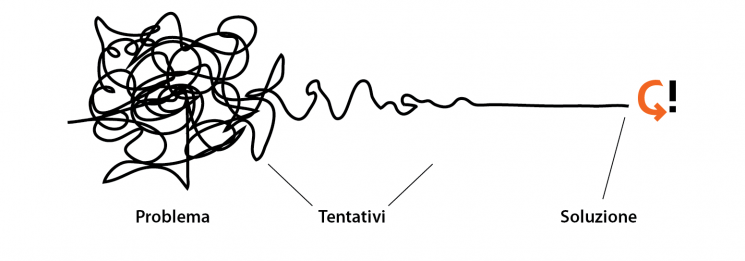
\includegraphics[width=\textwidth,keepaspectratio=true]{capitoli/imgs/Design-Thinking.png}
	\caption{Schematizzazione molto basilare del Design Thinking}
\end{figure}
\begin{itemize}
	\item Definire il problema \\
	In questa fase del lavoro è fondamentale osservare, capire le abitudini degli utenti ed immedesimarsi in loro.
	\item Divergere \\
	Quì entra in gioco la creatività, cercando di mettere sul piatto il maggior numero di soluzioni possibili, evitando però preconcetti sulle soluzioni e concentrandosi solamente sul problema.
	\item Testare \\
	E' necessario ora produrre dei prototipi testabili in modo che si possano comparare le diverse soluzioni e ricevere feedback dagli utenti.
	\item Convergere \\
	A questo punto è il tempo di dirigersi verso una soluzione, utilizzando anche la creatività per attuare dei compromessi tra quelle soluzioni parziali che intersecano al meglio i requisiti.
\end{itemize}


\subsection{BigFix SaaS Interaction Design}
Il nodo cruciale di questa fase del lavoro e stato per noi quello di capire realmente quale fosse il target del nuovo servizio SaaS e quali siano i reali bisogni che possano spingere i clienti ad adottare un prodotto SaaS, siano essi già degli utenti della versione on premise o no. Il problema principale prima dell'avvento del paradigma design thinking era che i requisiti funzionali dei prodotti che venivano realizzati per le aziende erano stabiliti tramite delle contrattazioni svolte tra i progettisti e gli addetti agli acquisti delle aziende clienti, spesso trascurando i reali beneficiari del prodotto, ossia i tecnici dell'azienda cliente. Questo spesso porta a realizzare dei prodotti che non fanno fronte ai reali bisogni dell'utente. 

\paragraph{}
La novità introdotta dal design thinking è il coinvolgimento della figura dell'utente finale fin dalla progettazione. Questo è stato fatto tramite interviste ma anche osservando gli utenti nella loro routine lavorative, cercando di captare necessità e frustrazioni che vogliono essere eliminate.

\paragraph{}
continuare quì

\section{Requisiti Non Funzionali}
Abbiamo già parlato nel capitolo 4 di quali sono le nuove problematiche alle quali una SaaS application deve far fronte. Ovviamente nel mio lavoro di tesi questo aspetto è stato un argomento cruciale delle prime fasi del lavoro. Soddisfare questo tipo di requisiti comporta infatti fare scelte architetturali molto impattanti e in quanto tali occorre definirle prima possibile nel design di un sistema software. 

\subsection{Dependability}
Il servizio di BigFix SaaS è stato progettato per garantire, quando sarà in produzione, un'availability che si mantenga sempre su valori superiori al 99. Ovviamente si prevedono carichi di utilizzo che possono essere anche molto elevati. La suite di BigFix è utilizzata contemporaneamente da clienti di tutto il mondo, alcuni dei quali possiedono una rete di endpoint composta da un numero considerevole di nodi. Tutto ciò può portare a picchi di carico molto elevati nonostante i quali il servizio deve continuare a essere disponibile con prestazioni sopra delle soglie minime di accettabilità.

\paragraph{Microservizi e container}
Come abbiamo potuto osservare nei capitoli precedenti, l'adozione di microservizi e container è un must per i servizi cloud. Grazie a questa scelta possiamo garantire agli utenti di BigFix SaaS un'alta Dependability, fattore fondamentale nel contesto della security aziendale in cui si va a calare questa suite di prodotti. I microservizi di BigFix, infatti, verranno replicati tramite i container in datacenter IBM in tutto il mondo, ciò potrà garantire anche tolleranza ai guasti che possono presentarsi. Il grado di replicazione dei diversi microservizi sarà ovviamente proporzionale all'importanza del microservizio stesso. Ci saranno ovviamente dei microservizi con dei ruoli più centrali di altri.

\subsubsection{Rolling Update}
Un'altro aspetto critico nel garantire un'alta availability è quello dell'aggiornamento del servizio. Facendo un paragone con i servizi SaaS che utilizziamo quotidianamente per consultare la posta elettronica, notiamo che non assistiamo mai a fenomeni di mancanza del servizio quando il prodotto si aggiorna, ma, all'occorrenza, troviamo già il prodotto nella sua versione agiornata. Vogliamo che questo comportamento si verifichi anche con la suite SaaS di BigFix e per questo occorre attuare una politica di Rolling Update. Silentemente, vengono aggiornate a turno tutte le repliche dei microservizi interessanti dall'aggiornamento. Nel fare ciò però, l'esperienza utente non risente di peggioramenti, in quanto le repliche che rimangono in servizio garantiscono l'efficienza del servizio.

\subsubsection{Utilizzo di BD2}
Anche la persistenza dei dati può risultare essere un elemento critico per la dependability. Occorre uno strumento che garantisca l'integrità dei dati, la resistenza ai guasti con adeguate misure di ripristino e soprattutto la riservatezza dei dati che, in un contesto come la security aziendale, possono essere molto sensibili. Si è scelto di utilizzare come DBMS DB2, un database relazionale prodotto da IBM. Una peculiarità di questo prodotto è la HADR (High Availability and Disaster Recovery). Diamo un'occhiata all'architettura di DB2 per capire di cosa si tratta.

\begin{figure}[h!]
	\centering
	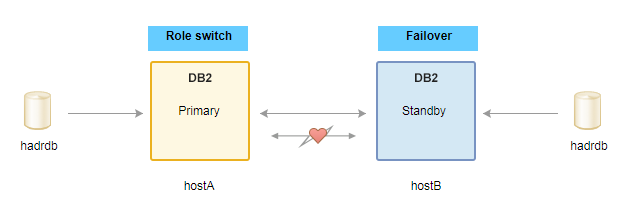
\includegraphics[width=\textwidth,keepaspectratio=true]{capitoli/imgs/db2.PNG}
	\caption{Architettura del DBMS IBM DB2}
\end{figure}

\paragraph{}
DB2 replica tutto il contenuto del suo database, chiamato Primary Database, in un secondo database detto Standby Database, il quale svolge anche il ruolo di backup. I dati di questi due sono consistenti e vengono sincronizzati costantemente. Qualunque malfunzionamento del database principale normalmente comporterebbe dei tempi di non availability più o meno lunghi. Con questa architettura HADR, invece, nel momento in cui il Primary Database presenta un guasto, lo Standby Database assume il suo ruolo (Failover) finchè il database primario non torna disponibile e, a qual punto, i due database tornano a svolgere il loro compito originario (Role switch). Una prerogativa importante però è che i due database risiedano in due data center distinti, o comunque provengano da due fonti di energia distinte nel caso si trovino nello stesso luogo geografico, per evitare che dei guasti possano colpirli entrambi. 

\subsection{Scalabilità}
Per quanto riguarda la Scalabilita ci prefiggiamo di garantire le stesse specifiche del prodotto in versione on premise, quindi di supportare fino a 250.000 endpoint per server. Il soddisfacimento di questa specifica, nel contesto SaaS, sposta l'attenzione ovviamente sul nuovo concetto di server, ossia una serie di microservizi distribuiti che svolgono le funzionalità che nella versione on premise era svolta dal server presso il client. Ancora una volta sta nella ridondanza dei microservizi la chiave per garantire la scalabilità prefissata.

\subsection{Monitoring}
Sotto l'aspetto del monitoring ci siamo dovuti scontrare con una nuova complessità nel saper monitorare un servizio così diffuso come quello di SaaS. La necessità è quella di sostituire l'intervento umano nella consultazione dei log di tutti i servizi. Il requisito che abbiamo è quello di analizzare i risultati, saper effettuare delle medie e calcolare dei picchi di parametri come il throughput o la latenza. Vogliamo infine che questa mole di dati fosse facilmente consultabile agli occhi di chi effettua la manutenzione del prodotto, magari sotto forma di grafici facilmente intellegibili. Per soddisfare queste necessità abbiamo individuato i tool Prometheus e Grafana che si sono rivelati molto utili nelle fasi successive al deployment, come vedremo in seguito.  


\section{Gap con il prodotto on premise}
La natura di un servizio SaaS porta con se alcune differenze strutturali importanti con il prodotto già esistente. La modalità di fruizione del prodotto è completamente diversa dal prodotto on premise infatti e gli accorgimenti sono da prendere subito in considerazione in quanto impattano pesantemente sulle scelte architetturali.
\paragraph{Introduzione della multitenancy}
Uno di questi è sicuramente la multitenancy. Nel modello SaaS può capitare che sulla stessa macchina fisica risiedano più server di clienti diversi. Dalla prospettiva utente però si deve dare l'impressione di un possesso esclusivo del server tramite strategie di multitenancy. E' di fondamentale importanza che un cliente non entri in contatto con dati afferenti al server di altre organizzazioni, anche se queste risiedono sullo stesso server fisico. Tra gli accorgimenti attuati c'è la modifica della modalità di archiviazione dei dati, permettendo di filtrare i dati appartenenti al tenant corretto e speciali privilegi di utilizzo dei servizi server. 
\paragraph{Introduzione dei microservizi}
L'introduzione dei microservizi è un elemento centrale della conversione a SaaS. Per attuarla è necessario un attento percorso di refactoring del codice del prodotto, suddividendolo in servizi coesi che possano rappresentare delle entità separate che cooperino tra loro.

\section{Definizione Architetturale}
La definizione di un'architettura di un prodotto così complesso è guidata da un'attenta analisi dei requisiti appena descritti. Occorre definire componenti ben definiti da implementare, altri da riutilizzare, alcuni da adattare e inoltre interfacciarsi con nuove tecnologie che devono essere opportunamente inserite nel contesto di applicazione.
\subsection{Scelta dei tool e dei servizi da utilizzare}
\subsection{Viste architetturali}
